% 1) Title
% 2) Date
% 3) Location
% 4) Present
% 5) Picture
% 6) Start Time
% 7) Stop Time
\insertmeeting 
	{Space Coast Meet \#2} 
	{12/18/21}
	{Odyssey Charter School}
	{Annika, Anouska, Clayton, Falon, James, Jensen, Nathan, Ritam, Rose, Samantha, Lilly}
	{Images/RobotPics/robot.jpg}
	{8:00 - 5:00}
	
\section*{The Rise of Scoopie}
\noindent\hfil\rule{\textwidth}{.4pt}\hfil
\subsection*{Goals}
\begin{itemize}
    \item Assess how we can improve Scoopie
    \item Look into different strategies for Shared Hub
    \item Reflect on our most recent competition at Odyssey Charter School, determining our strengths and failures

\end{itemize} 

\noindent\hfil\rule{\textwidth}{.4pt}\hfil

\subsection*{Accomplishments}
The Mechromancers had the second meet of the season December 18th at Odyssey Charter School, Florida. Our team ranked in 3rd place, with 4 wins and 2 losses. This meet was a lot more successful since the last meet considering the amount of points we earned improved since the last meet. Our strategy was considerably more thought out since the last meet. Upon reflection on this meet we discovered the intake needs considerable improvement in order to increase robots efficiency, especially since the current sporadic design tended to lead to penalties.  For the league championship, we want to budget our time more efficiently so that a minimal amount of time is spent on the larger changes to the hardware and the programers have more time to program to get a smoother running autonomous. The same applies to the drivers, as the largest cause of error within this meet was through the lack of driver practice. We have considered a solution, halting changes to the robot at least a week before the competitions so that the drivers can practice how to operate with the newly made changes.  
- Leave a week of practice for drivers to practice for all conditions that may occur at the competition
- Practice from both alliance sides to allow drivers to become more comfortable with the field perspectives
- Practice intaking freight to avoid the accidentally flinging of cargo and penalties. 
Improve intake efficiency considerably 

The first and most significant issue that we encountered was lack of driver practice. For Scoopie the connection between the driver and operator was vital as they must be timed perfectly in order to drop off the cargo successfully into the sharbed hub. More driver practice is also vital in order for Scoopie to take the corners around the field due to Scoopie’s inability to go over the barriers between the warehouses and the shipping hubs. In order to successfully maneuver around the sharp corners more driver practice is vital. Perhaps the programmers could potentially create a way to take the 90 corner better. This means that we must budget our time correctly in order to allow the programmers and the drive team time to work together to configure to work that out. The drivers also must from this point forward practice from both alliance sides in order to work out all the kinks with going around the corners.  We would also benefit by doing more matches with other robots to see how they might hinder Scoopie’s maneuverability. 
A  major hardware issue we encountered was that the intake was inefficient . Due to a mix of lack of practice and some programming issues the intake cost a lot of time and so we were not able to pick up as much cargo as we initially anticipated.




\begin{figure}[ht]
\centering
\begin{minipage}[b]{.48\textwidth}
  \centering
  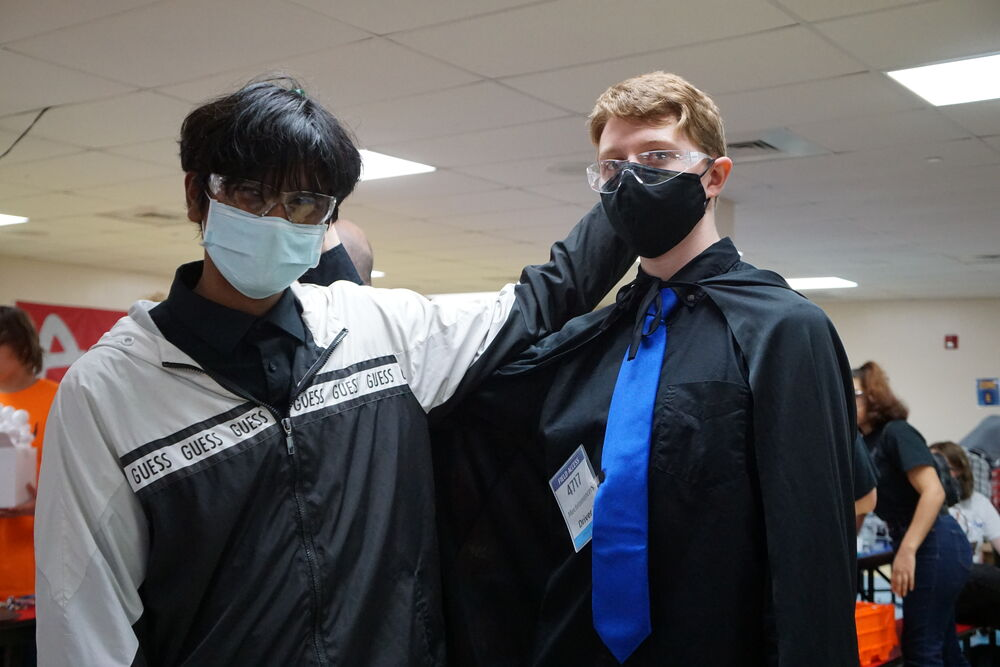
\includegraphics[width=0.95\textwidth]{Meetings/December/12-18-21/12-18-21_Team_Figure1 - Nathan Forrer.JPG}
  \caption{Samantha scouting the opponents}
  \label{fig:121821_1}
\end{minipage}%
\hfill%
\begin{minipage}[b]{.48\textwidth}
  \centering
  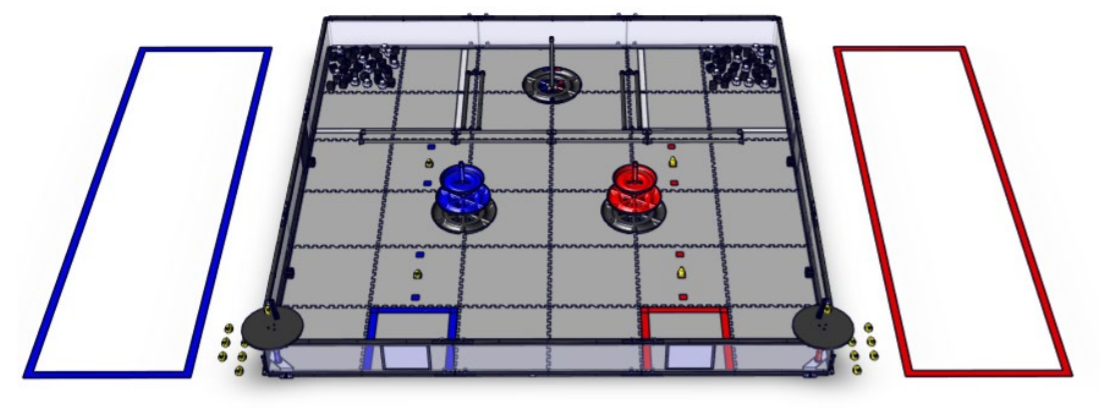
\includegraphics[width=0.95\textwidth]{Meetings/December/12-18-21/field.png}
  \caption{Anouska setting up the robot}
  \label{fig:121821_2}
\end{minipage}
\end{figure}

\begin{figure}[htp]
\centering
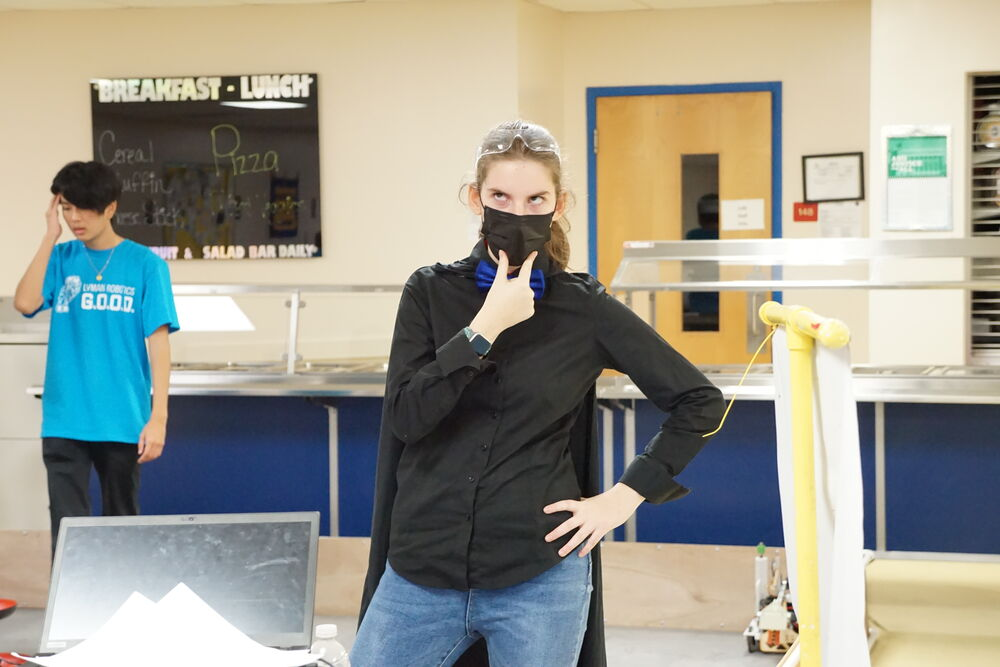
\includegraphics[width=0.95\textwidth, angle=0]{Meetings/December/12-18-21/12-18-21_Team_Figure3 - Nathan Forrer.JPG}
\caption{Ritam and Nathan posing for the camera}
\label{fig:121821_3}
\end{figure}


\whatsnext{
\begin{itemize}
    \item Laser cut intake parts
    \item 3d print intake parts
    \item Build intake
\end{itemize} 
}






